



\subsection{Possibilistic Variables}
A possibilistic variable $X$ over a universe $U$ is defined as a variable taking exactly one value in $U$, but for which this value is (partially) unknown. The possibility distribution $\pi_X$ gives the available knowledge about the value that $X$ takes. For each $u\in U$, $\pi_X(u)$ represents the possibility that $X$ takes the value $u$.

It is important to understand the difference between the following two concepts:
\begin{itemize}
\item
A \emph{possibilistic variable} $X$ is bounded to take only one value , but this value is not known due to incomplete knowledge. 
\item
An \emph{ill-known set}~\cite{Dubois88b}: a possibilistic variable defined over the universe $\Pow(U)$.
\end{itemize}

Note that while a possibilistic variable refers to one (partially) unknown value, an ill-known set is a crisp set but, for some reason, (partially) unknown.


\subsection{\label{subsec:fuzzy-numbers}Fuzzy numbers and fuzzy intervals}
Dubois and Prade~\cite{Dubois1983} proposed the following definition of \emph{fuzzy interval}.
%\begin{definition}
A fuzzy interval is a fuzzy set $M$ on the set of real numbers $\mathbb{R}$ such that:
\begin{eqnarray}
\forall (u,v)\in\mathbb{R}^2:&\\
\nonumber
\forall w \in [u,v]:&\mu_M(w) \geq\min(\mu_M(u),\mu_M(v))  \\
\exists m \in \mathbb{R}:& \mu_M(m)=1 
\end{eqnarray}
%\end{definition}
If $m$ is unique, then $M$ is referred to as a \emph{fuzzy number}, instead of a \emph{fuzzy interval}. In other words, if the core of a fuzzy interval is a singleton, it can be seen as a fuzzy number. In their work, Dubois and Prade propose four different functions (two possibility and two necessity functions) to asses the position of a fuzzy number N relative to  a fuzzy number M taken as a reference.

The most convenient representation for the membership function of a fuzzy number is a triangular function. The membership function $\mu_M$ for the fuzzy set $M$ has also the properties of convexity and normalization. Three values represent a triangular function (see Figure~\ref{fig:triangular}):
\begin{itemize}
\item
$D$ is the singleton value in the core of $\mu_M(x)$.
\item
$D-a$ is the lower value in the support of $\mu_M(x)$. 
\item
$D+b$ is the upper value in the support of $\mu_M(x)$.
\end{itemize}
Note that the values $a$ and $b$ are values in the underlying ordered domain. E.g. $(a,b) \in \mathbb{R}^2$. The notation for a triangular function adopted here is $[D,a,b]$.
\begin{figure}[h!]
  \centering
  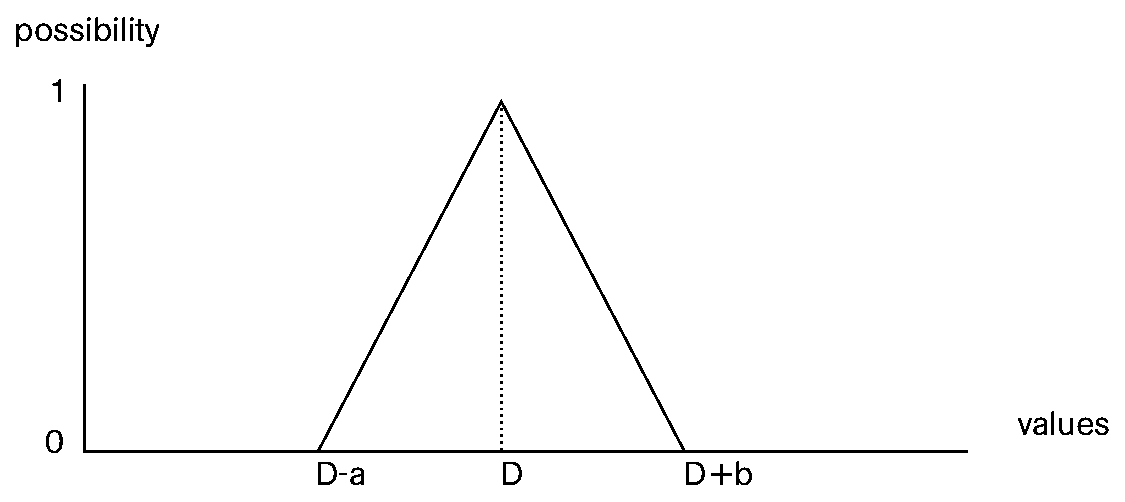
\includegraphics[scale=0.4]{graphs/triangular.eps}
  \caption{Triangular function.}
  \label{fig:triangular}
\end{figure}

The most simple representation for the membership function of a fuzzy interval is a trapezoidal function. This membership function $\mu_T$ for the fuzzy interval $T$ is convex and normalized. Four values represent a trapezoidal membership function (figure  \ref{fig:trapezoidal}): $\left[\alpha,\ \beta,\ \gamma,\ \delta\right]$. The membership function is given by:

\begin{align}
\mu_T(x)
\begin{cases}
1 & \mbox{ if } x \in [\beta,\gamma] \\
0 & \mbox{ if } x > \delta \vee x < \alpha \\
\frac{x-\alpha}{\beta - \alpha} & \mbox{ if } x \in [\alpha,\beta[ \\
\frac{\delta -x}{\delta - \gamma} & \mbox{ if } x \in ]\gamma,\delta] \\
\end{cases}
\end{align}

\begin{figure}[h!]
  \centering
  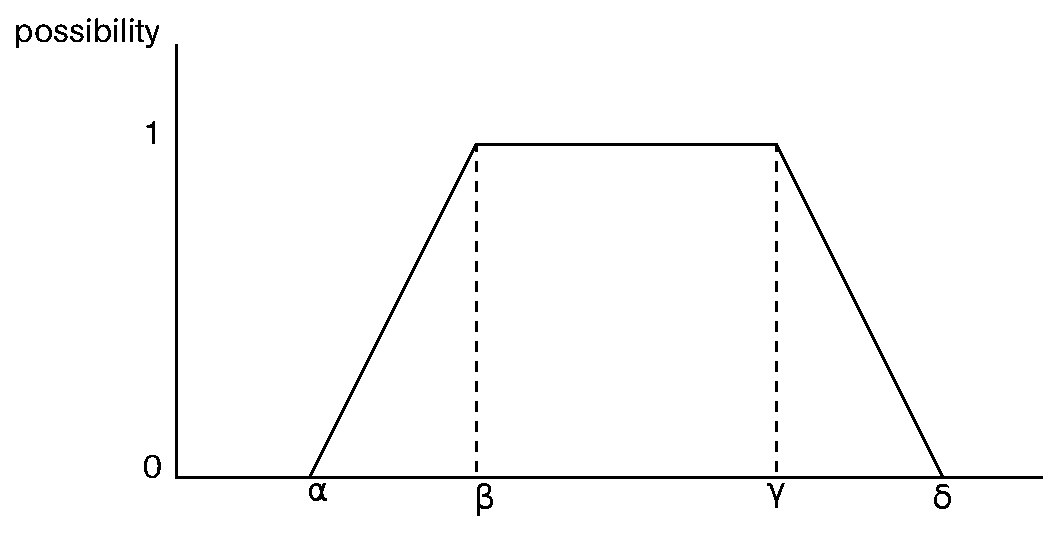
\includegraphics[scale=0.4]{graphs/trapezoidalDistribution.eps}
  \caption{Trapezoidal distribution.}
  \label{fig:trapezoidal}
\end{figure}

\subsubsection{Set evaluation by ill-known constraints}

\subsubsection{Interval evaluation by ill-known constraints}
The problem of the interval evaluation is explained in \cite{Pon11}: For a crisp interval $I = \left[ a, b \right]$, we want to know if all points in this interval reside between the boundaries of the ill-known interval $\left[ X , Y \right]$, where $X,Y$ are ill-known values on the set of real numbers $\mathbb{R}$, and $\lambda$ is the evaluation function. The following expressions compute the possibility and the necessity: 

\begin{eqnarray}
\label{eq:interval-pos}
\Pos\left(\lambda([a,b])\right)=\\
\nonumber
\min\bigg(\sup_{a\geq w}\pi_{X}(w),\sup_{b\leq w}\pi_{Y}(w)\bigg)\\
\label{eq:interval-nec}
\Nec\left(\lambda([a,b])\right)=\\
\nonumber
\min\bigg(\inf_{a<w}1-\pi_{X}(w),\inf_{b>w}1-\pi_{Y}(w)\bigg).
\end{eqnarray}

\paragraph{Example} Consider the ill-known values $X = \left[5, 2, 8\right]$ and $Y = \left[9, 7, 10 \right]$. The knowledge about the evaluation of the interval $\left[a, b \right]$  is given by the expressions \eqref{eq:interval-pos},\eqref{eq:interval-nec}.  Figure~\ref{fig:3d-possibility} shows a 3D plot of the possibility that an interval $[a,b]$ passes the evaluations specified by the ill-known constraints. Note the triangular form for the resulting possibility distribution since the condition $a \leq b$ holds.

\begin{figure}[h!]
\centering
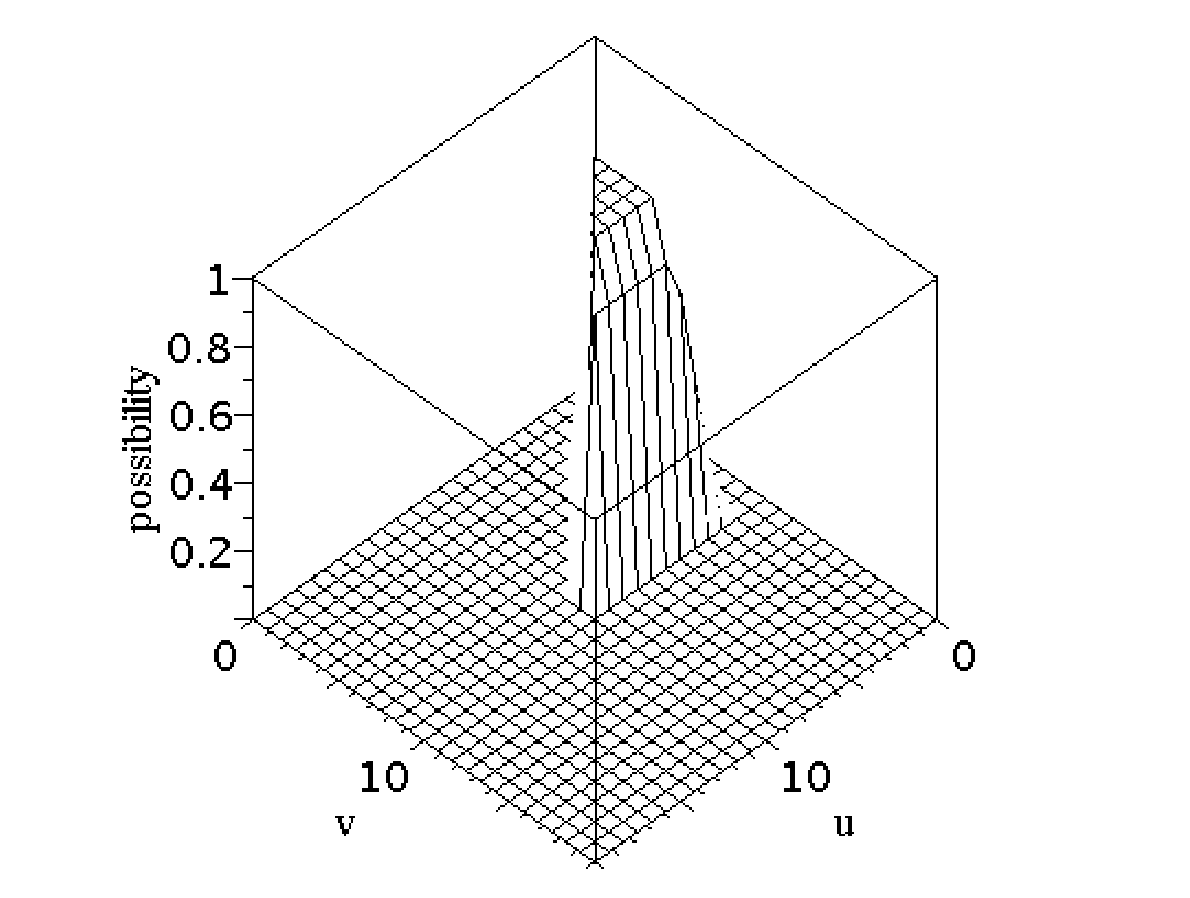
\includegraphics[scale=0.4]{graphs/3D_possibility.eps}
\caption{Possibility of evaluation for the interval $[a,b]$.}
\label{fig:3d-possibility}
\end{figure}
The necessity plot is obtained in a similar way and is shown in Figure~\ref{fig:3d-necessity}. Notice that the necessity measure is not normalized because the supports of $X$ and $Y$ overlap.
\begin{figure}[h!]
\centering
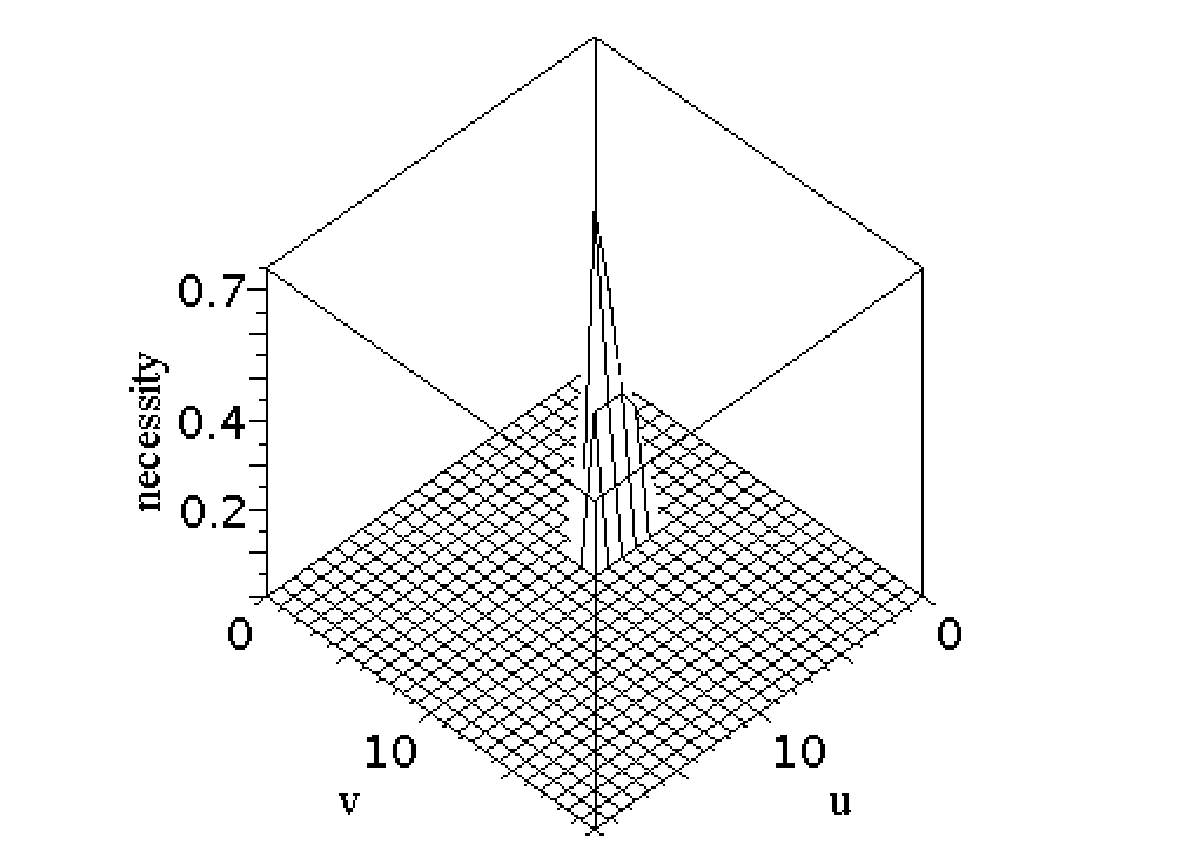
\includegraphics[scale=0.4]{graphs/3D_necessity.eps}
\caption{Necessity of evaluation for the interval $[a,b]$.}
\label{fig:3d-necessity}
\end{figure}



\subsection{Temporal databases}
%In this section, the proposed reasoning is applied to the specific context of intervals on the real line. This setting is of specific interest in the context of fuzzy temporal databases.
A temporal database \cite{Dyreson1994} is a database that manages some aspects of time in its schema. A \textbf{chronon} is the shortest duration of time supported by the database. The time can be represented either as points or intervals \cite{655777}. Fuzzy temporal models \cite{4481150} are proposed when the time points or intervals are not precisely known. There are proposals for the  fuzzyfication of the time point \cite{Dubois89} and the fuzzyfication of the time interval \cite{Garrido2009}.\\
Allen \cite{Allen:1983:MKT:182.358434} studied the comparison between two crisp time intervals. For fuzzy intervals, several proposals \cite{4481150}, \cite{springerlink:10.1007/978-3-540-39964-3_57},\cite{10.1109/TIME.2004.1314418} have been done.


%Time granularity is also associated with the representation of the time. A granularity is the result of partitioning on the set of chronons. The conversion among granularities is a common issue within temporal databases \cite{Lin97efficientconversion}. Granularity is the basis of some systems \cite{Cru97},\cite{624013}.


Despite of user-defined time (an uninterpreted attribute; supported in the standard SQL2 \cite{Mel93}), there are 3 types of time in a temporal database:

\begin{itemize}
	\item
	\textbf{Transaction time}: The time when the fact is stored in the database.
	\item
	\textbf{Valid time}: The time when the fact is true in the modelled reality.
	\item
	\textbf{Decision time} \cite{Nascimento95decisiontime}: The time when an event was decided to happen. 
	\end{itemize}
	
	 The  database model can be then classified into: transaction time \cite{Ston87},\cite{Jensen:1991:IIM:627283.627484}, Valid time, bi-temporal \cite{Snodgrass:1984:TQL:588011.588041}(both valid and transaction time) or tri-temporal \cite{Nascimento95decisiontime} (valid, transaction and decision time).

Fuzzy temporal models \cite{4481150} deal with time points \cite{Dubois89} or intervals \cite{Garrido2009} that are ill-known. Some fuzzy temporal models assume that the time stored in the database is an interval. The temporal interval is represented by two ill-known time points: $X$  an ill-known starting point and $Y$ an ill-known ending point. The interval $\left[X,Y\right]$ is not a fuzzy interval but an ill-known interval: it is a crisp interval but it is partially unknown which values are in this interval.
